\begin{problem}{5} ~\\
(a) If f(f(p)) = p, Algorithm B gives a factor of two approximation. If f(f(p)) is any point other than p, then the distance from f(p) to f(f(p)) must be greater than the distance from p to f(p). Therefore, Algorithm B always gives an approximation factor or two or better.\\
\\
(b) In one dimension, no matter which p is picked, f(p) will always be the point on the left or right side. Then f(f(p)) will always be the point on the other side to f(p). The distance from f(p) to f(f(p)) (from the left/right side to the right/left side) is the exact diameter for the set.\\
\\
(c)\begin{figure}[H] 
\centering 
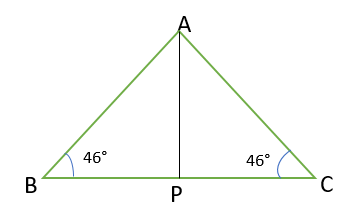
\includegraphics[width=0.6\columnwidth]{1}
\end{figure}
Illustrated by the above graph, ABC is an isosceles triangle, P is the midpoint of BC. Let p = P, then f(p) would be A, f(f(p)) would be either B or C. In fact, the diameter of the point set \{A,B,C,P\} is BC. Therefore, Algorithm B does not always produce the correct diameter in two dimensions.\\
\\
(d) To guarantee the approximation factor, we need to find the shortest possible distance that Algorithm B can find. In other words, we need to find the Min(d(f(P), f(f(P))). Suppose that AB is the optimal distance of a graph and AB = 2, then in the worst case, f(P) $\neq$ A/B and f(f(P)) is either P or A or B, as shown by the graph below. The blue line illustrates the bisector of AB.
\begin{figure}[H] 
\centering 
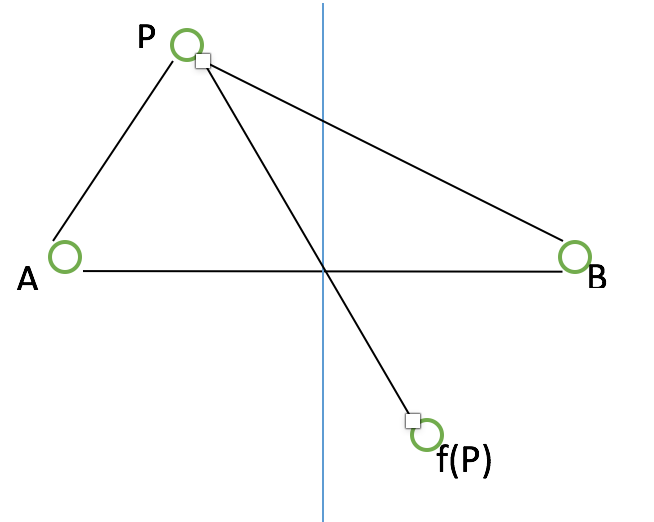
\includegraphics[width=0.5\columnwidth]{2}
\end{figure}
To get the Min(d(f(P), f(f(P))), MAX(PA, PB) = Pf(P) (here we suppose PB = Pf(P)), and f(P) and P have to be on the bisector.\\
\\
Proof: If we make no assumption on the position of P, then d(f(P), A) would be minimized when f(P) is on the bisector under the condition that PA $\leq$ PB and PB = Pf(P).\\
\\
The above proof also works for P, because when P is on the bisector, MAX(PA, PB) would be minimized, which means d(P, f(P)) is minimized. In other words, when both P and f(P) are on the bisector, the three possible choices of d(f(P), f(f(P))): d(P, f(P)), MAX(d(f(P), A), d(f(P), B)) are all minimized.\\
\begin{figure}[H] 
\centering 
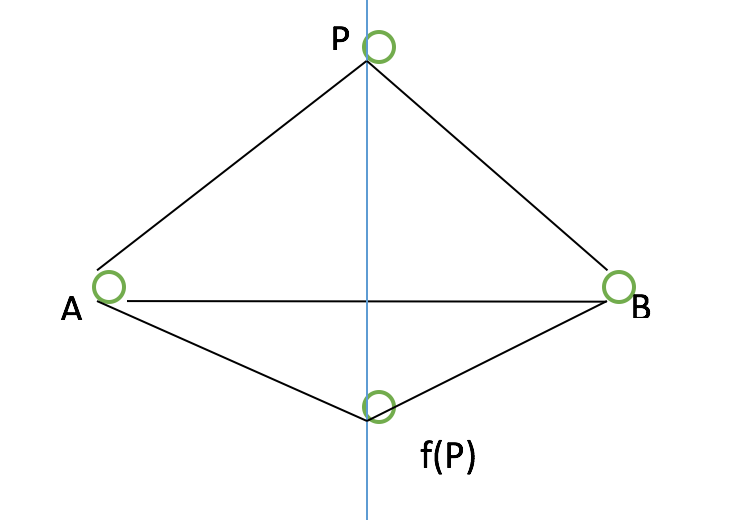
\includegraphics[width=0.5\columnwidth]{3}
\end{figure}
Now what we need to do is comparing d(P, f(P)) and d(f(P), B) based on all the restrictions mentioned above (e.g. d(P, f(P)) = d(P, B)). When d(P, B) = d(P, f(P)) = d(f(P), B), MAX(d(P, f(P)), d(f(P), B)) = $\frac{2\sqrt[]{3}}{3}$ reaches the minimum. Therefore the approximation factor is guaranteed to be at most $\sqrt[]{3}$.
\end{problem}